
\section{Method}
\label{sec:method}
In this section, we introduce the problem setting formally and we lay out the LIDL method theoretically, including its derivation and pointing out certain predictions about its behavior that we later verify empirically in Section~\ref{sec:empirical-evaluation}.

It is often known that a particular dataset $X$ is a subset of some data manifold $M$ equipped with probability measure $\mu$. However, the manifold $M$ and the dataset $X$ need not be directly observable. Instead, there may exist an embedding (or, more generally, an immersion satisfying some regularity conditions, see Appendix~\ref{sec:non-connected}) $j\colon M\to\R^D$ into a Euclidean space of larger dimension, through which we can view $X$. 

The method we propose is based upon the observation, expressed in Theorem~\ref{thm:core-estimate}, that for a probability measure supported on an embedded submanifold of an Euclidean space, the dimension of its support can be recovered from its asymptotic behavior under small normally distributed perturbations (see Fig.~\ref{fig:method-1} for an intuitive illustration). 

\subsection{The formal setting}

We first define a class of measures we will restrict our considerations to, which we will call \emph{smooth} measures, including all measures with continuous positive densities.

\begin{definition}
\label{def:smooth-measure}
    A positive measure $\nu$ on a manifold $N$ will be called \emph{smooth} if for any chart $\psi\colon U\to V\subset\R^n$ of $N$, the pushforward $\psi_*\nu$ is absolutely continuous with respect to the Lebesgue measure $\lambda$ on $V$, and moreover, its density is locally bounded away from $0$, i.e.\ any $x\in V$ admits a neighborhood on which $dj_*\nu/d\lambda > c$ for some $c>0$.
\end{definition}


Let $S\subset\R^D$ be a smooth connected  $d$-dimensional embedded submanifold of a high-dimensional Euclidean space $\R^D$ (the more general case of a non-connected immersed manifold is dealt with in Appendix~\ref{sec:non-connected}).
This is our observable data manifold, embedded in Euclidean space, i.e.\ $S=j(M)$. Furthermore, suppose we are given a smooth (according to Definition~\ref{def:smooth-measure}) probability measure $p_S$ on $S$, representing the data probability distribution. In our notation, this is the pushforward of the probability $\mu$ on $M$, i.e.\ $p_S = j_*\mu$. We will implicitly treat $p_S$ as a probability distribution on the whole ambient space $\R^D$.

The Gaussian function (i.e.\ the density of the standard normal distribution) on a Euclidean space $V$ will be denoted by $\phi^V$, or $\phi^n$ in the case where $V$ is the standard $\R^n$ space. Also, for $\delta > 0$, let
\begin{equation}
\label{eq:dilated-gaussian}
    \phi^V_{\delta}(x) = \delta^{-\dim V}\phi^V(x/\delta)
\end{equation} 
be the density of the normal distribution $\N(0, \delta^2 I)$ with covariance matrix $\delta^2 I$, where $I$ is the identity matrix on $V$. 
 
Under the above notation, if $X\sim p_S$ is a random vector representing the data, and $N_\delta\sim\N(0,\delta^2 I)$ a normally distributed random noise vector, the distribution of the perturbed random vector $X+N_\delta$ in $\R^D$ is given by the convolution $p_S * \N(0,\delta^2 I)$, and has density
\begin{equation}
\label{eq:mollified-density}
    \rho_\delta(x) = \int_S \phi^D_{\delta}(x-y)\, d p_S(y).
\end{equation}

Finally, let us introduce a notation for uniform multiplicative estimates. We will write that $f(x,y) \asymp g(x,y)$ uniformly in $x$ if for every $y$ there exists $C>0$ such that for all $x$
\begin{equation}
    C^{-1}g(x,y) \leq f(x,y) \leq Cg(x,y).
\end{equation}
This notation extends to any number of variables. We will use it to declutter the proofs from irrelevant 
constants.


\subsection{The core estimate}
\label{sec:core-estimate}


At any $x\in S$ the tangent space of $\R^D$ admits a decomposition $T_x\R^D = T_xS \oplus N_xS$ into a direct sum of the tangent and normal spaces of $S$. Under the natural identification of $T_x\R^D$ with the underlying $\R^D$ (mapping the origin of $T_xS$ to $x$), the tangent and normal spaces of $S$ at $x$ become two affine subspaces of $\R^D$ intersecting at $x$. Denote by $\pi_x\colon \R^D\to T_xS$ and $\pip_x\colon \R^D\to N_xS$ be the corresponding orthogonal projections. With this notation, the following decomposition of the Gaussian density holds
\begin{equation}
\label{eq:gaussian-decomposition}
    \phi^D_\delta(x-y) = \phi^{T_xS}_\delta(\pi_x(y)) \phi^{N_xS}_\delta(\pip_x(y)).
\end{equation}

By the Inverse Function Theorem applied to the restriction of $\pi_x$ to $S$, in a small neighborhood of any $x\in S$, the manifold $S$ can be represented as the graph of a smooth map $F_x\colon T_xS \to N_x S$. In particular, it follows that in this neighborhood one has $\pip_x = F_x \circ \pi_x$. Moreover, $F_x(0) = 0$, and since the graph of $F_x$ is tangent to $T_xS$ at the origin, the derivative of $F_x$ at $x$ vanishes. Hence, the Taylor expansion of $F_x$ at $0$ starts with the second-order term, and consequently, there exists $C>0$ such that for small $v$ 
\begin{equation}
\label{eq:local-parametrization-norm-estimate}
    \norm{F_x(v)}_{N_xS} \leq C\norm{v}_{T_xS}^2.
\end{equation}

We will precede the statement of the core estimate (Theorem~\ref{thm:core-estimate}) with five lemmas required for its proof. Denote by $B(x,r)$ the ball of radius $r$ in $\R^D$, centered at $x$. 

\begin{lemma}
\label{lem:ball-containment}
    Let $x\in S$. For sufficiently small $\delta$ the projection $\pi_x(S\cap B(x,\delta^{1/2}))$ contains the ball $B(x,\delta) \cap T_xS$. 
\end{lemma}

\begin{proof}
\label{lem:ball-containment-proof}
    Assume that $\delta$ is sufficiently small for $F_x$ to be defined on $B(x,\delta) \cap T_xS$. Let $v\in B(x,\delta) \cap T_xS$. Under our identifications, $y=(v,F_x(v)) \in T_xS \oplus N_xS$ is a point of $S$ such that $v=\pi_x(y)$. Moreover, by eq.~\eqref{eq:local-parametrization-norm-estimate}, for sufficiently small $\delta$
    \begin{equation}
        \norm{v}^2_{T_xS} + \norm{F_x(v)}^2_{N_xS} \leq \delta^2(1+ C\delta^2) < \delta,
    \end{equation}
    so $y\in B(x,\delta^{1/2})$, and $v \in \pi_x(S\cap B(x,\delta^{1/2}))$.
\end{proof}

\begin{lemma}
\label{lem:tangent-gaussian-estimate}
    For $x\in S$ and sufficiently small $\delta$, the estimate
    \begin{equation}
        \int_{S\cap B(x,\delta^{1/2})} \phi^{T_xS}_\delta(\pi_x(y))\,dp_S(y) \asymp 1
    \end{equation}
    holds uniformly in $\delta$.
\end{lemma}

\begin{proof}
    Denote $B=S\cap B(x,\delta^{1/2})$. Integrating by substitution, we obtain
    \begin{equation}
        \int_B \phi^{T_xS}_\delta(\pi_x(y))\,dp_S = \int_{\pi_x(B)}\phi^{T_xS}_\delta(v) \,d(\pi_x)_*p_S,
    \end{equation}
    where the pushforward $(\pi_x)_*p_S$ is a smooth measure on $T_xS$. Hence, for sufficiently small $\delta$
    \begin{equation}
    \label{eq:approximating-integral-of-tangential-normal-distribution}
        \int_{\pi_x(B)} \phi^{T_xS}_\delta(v) \,d(\pi_x)_*p_S(v) \asymp \int_{\pi_x(B)} \phi^{T_xS}_\delta(v) \,dv
    \end{equation}
    uniformly in $\delta$. The integral on the right is at most $1$, and simultaneously, by Lemma~\ref{lem:ball-containment} we have
    \begin{equation}
        \int_{\pi_x(B)} \phi^{T_xS}_\delta(v) \,dv \geq \int_{B(x,\delta)\cap T_xS} \phi^{T_xS}_\delta(v) \,dv.
    \end{equation}
    The last integral is the probability that a normal random variable falls within one standard deviation from the mean, which is a constant independent of $\delta$.
\end{proof}

\begin{lemma}
\label{lem:normal-gaussian-estimate}
    For sufficiently small $\delta$ and $y\in S\cap B(x, \delta^{1/2})$, where $x\in S$, the estimate $\phi^{N_xS}_\delta(\pip_x(y)) \asymp \delta^{d-D}$ holds uniformly in $\delta$ and $y$.
\end{lemma}

\begin{proof}
    By eq.~\eqref{eq:dilated-gaussian}, 
    \begin{equation}
        \phi^{N_xS}_\delta(\pip_x(y)) = \delta^{d-D}\phi^{N_xS}(\delta^{-1}\pip_x(y)).
    \end{equation}
    Since $\pi_x$ is a contraction, we have $\norm{\pi_x(y)} \leq \delta^{1/2}$. It follows from eq.~\eqref{eq:local-parametrization-norm-estimate}, that for sufficiently small $\delta$
    \begin{equation}
        \norm{\pip_x(y)} = \norm{F_x(\pi_x(y))} \leq C\delta
    \end{equation}
    for some $C>0$. Therefore $\delta^{-1}\pip_x(y)$ lies inside a fixed ball independent of $\delta$, and in consequence
    \begin{equation}
        \phi^{N_xS}(\delta^{-1}\pip_x(y)) \asymp 1
    \end{equation}
    uniformly in $\delta$, concluding the proof.
\end{proof}

\begin{lemma}
\label{lem:gaussian-estimate-on-ball}
    For $x\in S$ and sufficiently small $\delta$,
    \begin{equation}
        \int_{S\cap B(x,\delta^{1/2})} \phi^D_\delta(x-y)\, dp_S(y) \asymp \delta^{d-D}
    \end{equation}
    uniformly in $\delta$.
\end{lemma}

\begin{proof}
    Denote $B=S\cap B(x,\delta^{1/2})$. By eq.~\eqref{eq:gaussian-decomposition} and Lemma~\ref{lem:normal-gaussian-estimate}, for sufficiently small $\delta$ and $y\in B$, we have
    \begin{equation}
        \phi^D_\delta(x-y) \asymp \delta^{d-D} \phi^{T_xS}_\delta(\pi_x(y)) 
    \end{equation}
    uniformly in $\delta$. It follows that the original integral can be estimated as
    \begin{equation}
        \int_B \phi^D_\delta(x-y)\, dp_S \asymp \delta^{d-D} \int_B \phi^{T_xS}_\delta(\pi_x(y)) \, dp_S.
    \end{equation}
    The proof concludes by applying Lemma~\ref{lem:tangent-gaussian-estimate} to the last integral. 
\end{proof}

\begin{lemma}
\label{lem:gaussian-estimate-outside-ball}
    For every $x\in S$ 
    \begin{equation}
       \lim_{\delta\to 0^+}\,\int_{S\setminus B(x,\delta^{1/2})} \phi^D_\delta(x-y)\, dp_S(y) = 0.
    \end{equation}
\end{lemma}

\begin{proof}
    Observe that if $\norm{v} \geq \delta^{1/2}$, we have
    \begin{equation}
        \phi^D_\delta(v) \asymp \delta^{-D} \exp \left(-\frac{\norm{v}^2}{2\delta^2}\right) \leq \delta^{-D}\exp\left(-\frac{1}{2\delta}\right)
    \end{equation}
    uniformly in $v$. This bound on the integrand converges to $0$ as $\delta\to 0$, and the measure $p_S$ is finite, proving the convergence of the considered integral.
\end{proof}

\begin{theorem}[The core estimate]
\label{thm:core-estimate}
    Assume that $S \subset \R^D$ is a connected $d$-dimensional submanifold endowed with a smooth probability measure $p_S$. Let $\rho_\delta$ be the density of $p_S * \N(0, \delta^2 I)$ on $\R^D$. Then for $x\in S$ and sufficiently small $\delta$, we have
    \begin{equation}
    \label{eq:core-estimate}
        \log\rho_\delta(x) = (d-D)\log\delta + O(1).
    \end{equation}
\end{theorem}

\begin{proof}
    Since $\delta^{d-D}\geq 1$ for $\delta \leq 1$, given sufficiently small $\delta$, from Lemma~\ref{lem:gaussian-estimate-outside-ball} we get
    \begin{equation}
        \int_{S\setminus B(x,\delta^{1/2})} \phi^D_\delta(x-y)\, dp_S(y) < 
        \delta^{d-D}.
    \end{equation}
    By combining this with eq.~\eqref{eq:mollified-density} and Lemma~\ref{lem:gaussian-estimate-on-ball}, we obtain $\rho_\delta(x) \asymp \delta^{d-D}$, which yields the desired 
    estimate after taking $\log$.
\end{proof}



\subsection{The LIDL algorithm} 

\begin{algorithm}[b]
\caption{LIDL algorithm}
\label{alg:lidl}
\begin{algorithmic}
\REQUIRE
    $X\subset \R^D$; %
    $x_1,\dots, x_m \in\R^D$;  %
    $\delta_1, \dots, \delta_n \in \R^+$;  %
   
    
    
    
    \FOR{$j=1$ to $n$}
        \STATE $\DD_j \gets$ $\DD$ perturbed with $\N(0, \delta_j^2 \I_D)$ 
        \STATE Fit the density model $\hat\rho_j$ to $\DD_j$
    \ENDFOR
    \FOR{$i=1$ \TO $m$}
        \FOR{$j=1$ \TO $n$}
            \STATE $\xi_j \gets \log\delta_j$
            \STATE $\eta_j \gets \log\hat\rho_j(x_i)$
        \ENDFOR
        \STATE $\beta \gets$  regression coefficient for a set of $n$ points $(\xi_j, \eta_j)$
        \STATE $\hat{d}_i \gets D + \beta$
    \ENDFOR
    \STATE \textbf{return} $(\hat{d}_1, \dots, \hat{d}_m)$
\end{algorithmic}
\end{algorithm}

Now, let us consider how to use the core estimate derived above in practice. 
The core requirement of LIDL is access to the approximate densities $\rho_\delta(x)$, which we have to obtain by fitting a density estimator on the data points from the dataset perturbed with a normally distributed noise of an appropriate magnitude $\delta$. 
Luckily, these days there exist density estimators which scale to data even as high-dimensional as images.
For the purpose of empirical evaluation of our method, in this work we use three models from the family of NF, however we emphasize that our method could use absolutely any density estimation method.
A viable alternative could be, for example, using diffusion models \citep{song2021maximum}, which are likely to lead to further improved accuracy of LIDL estimates.


Given a dataset $\DD\subset\R^D$, and a point $x\in\R^D$, at which we want to estimate LID (usually $x\in D$, as we want to take a point from the image of the data manifold in $\R^D$), we proceed as follows. First, we choose $n>1$ values $\delta_1, \dots, \delta_n$ of perturbation magnitude. We discuss how to choose $\delta$ in the following section. Then, we fit $n$ probability densities $\hat\rho_i$, which will be our approximations of $\rho_{\delta_i}$. Having estimated the densities $\hat\rho_i$, we consider the sequence of points of the form $(\log \delta_i, \log\hat\rho_i(x))$. Using linear regression to fit eq.~\eqref{eq:core-estimate}, we get an estimate $\beta$ for $d-D$, from which we obtain $\hat{d} = D + \beta$, an estimate for $d$. To estimate LID for multiple points, we can fit the densities once, and then loop over the points. 
Full algorithm is presented in Algorithm \ref{alg:lidl}.

It is worth noting that our method fits nicely into the LID estimation framework presented in \cite{amsaleg2019intrinsic}. Roughly speaking, it is based on two observations. Firstly, the dimension of an Euclidean space can be recovered from the degree of the polynomial growth rate of its ball volume as a function of its radius. Secondly, this idea can be applied to discrete datasets by replacing the notion of ball volume with the likelihood function of finding a point of the dataset within a given distance from a fixed base point. 

In our notation, this likelihood function is $r\mapsto p_S(B(x,r))$, where $x$ is the base point. With reasonable assumptions on the measure $p_S$, it can be shown that for small $r$ this function behaves like a polynomial of degree $d$, so the LID value we are estimating is the same as what is defined in \cite{amsaleg2019intrinsic}, which can be consulted for more details.







\begin{figure}[b]
    \centering
    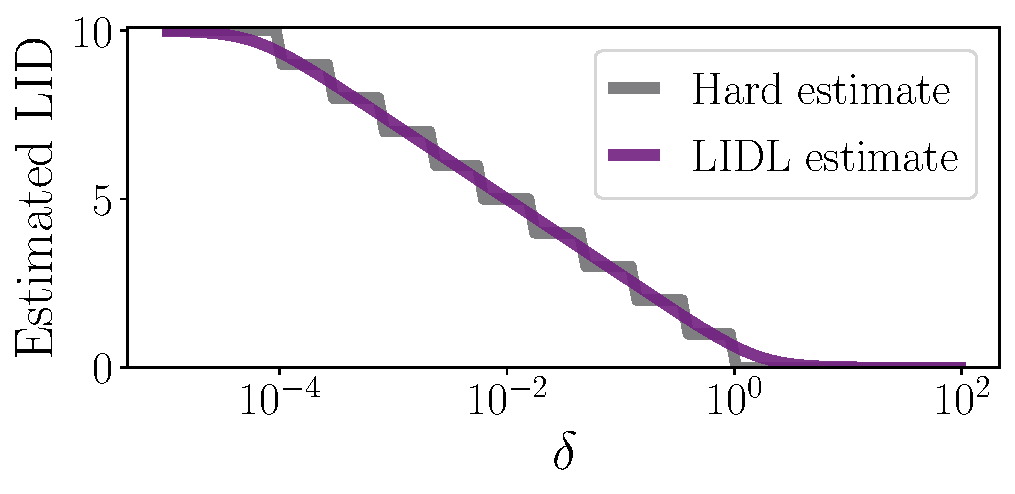
\includegraphics[width=0.4\textwidth]{images/step-delta-exp.pdf}
    \caption{LIDL and hard estimates for different values of $\delta$ for 10D non-isotripic Gaussian. Notice how LIDL ignores dimensions smaller than $\delta$, as predicted theoretically.}
    \label{fig:step-delta-exp}
\end{figure}

\subsection{Viewing $\delta$ as a scale parameter}
\label{sec:scale}



In the previous section, we glossed over the fact that we have to choose the values of $\delta$.
From Sec.~\ref{sec:core-estimate} we know that the core estimate is exact for infinitesimally small $\delta$, so the first pressure is for the $\delta$ to be small, possibly as small as the numerical precision allows. 

\begin{figure}[t]
    \centering
    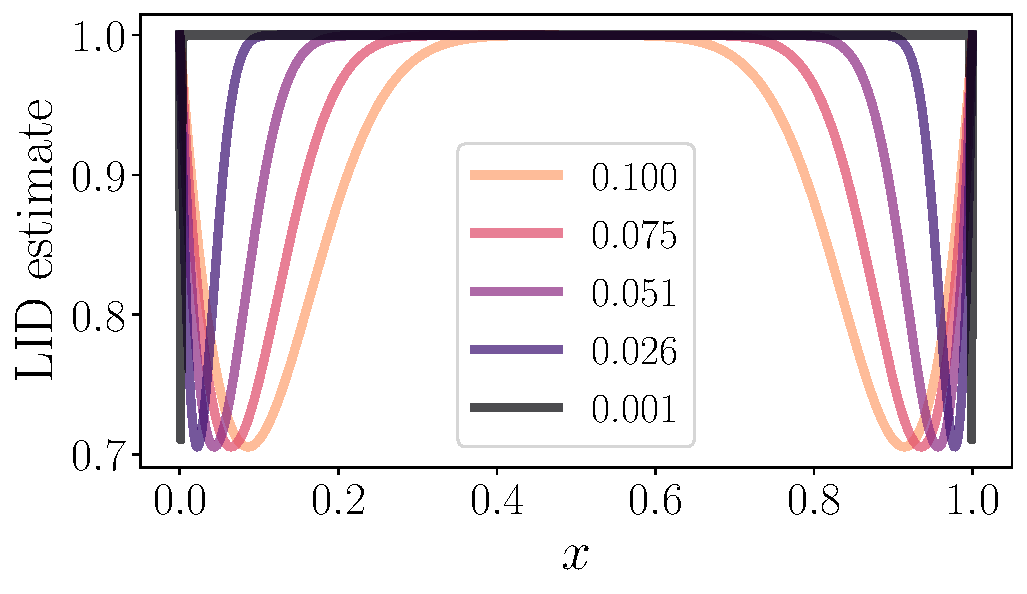
\includegraphics[width=0.4\textwidth]{images/evaluation-uniform.pdf}
    \caption{LIDL estimates for points from $\U(0,1)$ for different values of $\delta$ marked with different colors, as explained in the legend of the plot.}
    \label{fig:evaluation-uniform}
\end{figure}

However, $\delta$ can also be viewed as a length-scale parameter that allows users to choose a certain minimum `thickness' to be considered, such that dimensions `thinner' than the threshold will be ignored.
Consider an illustrative example:
suppose that the probability distribution $p_S$ is concentrated in a tubular neighborhood of another submanifold $S'$ of dimension $d'<d$. 
In this case, it can be approximated by a probability distribution $p_{S'}$ supported on $S'$.

Now, if this approximation is `good', in the sense that the thickness of the considered neighborhood is much smaller than the values of $\delta$ used, then intuitively the LIDL estimate should actually reflect the dimension $d'$ of the submanifold $S'$ instead of the true dimension $d$.

Continuing this example, 
we present the described behavior empirically. 
Let $S=\R^D$, and $p_S = \N(0, \Sigma)$, where $\Sigma$ is a diagonal matrix with entries $\sigma_1^2 \geq \sigma_2^2 \geq\dots\geq \sigma_D^2$. 
In Fig.~\ref{fig:step-delta-exp}, we plot the LIDL estimates for case $D=10$ and for $\sigma$ equally distributed on the logarithmic scale. We also plot the \emph{hard estimate} which is simply counting the number of entries in $\sigma$ that are larger than $\delta$. The LIDL estimate follows the hard estimate, and this behavior is predicted theoretically in Appendix~\ref{sec:appendix-lidl-for-normal-distribution}. 
We further investigate the role of the scale parameter in the case of imperfect density estimates in Sec.~\ref{sec:operating-range}.


As mentioned earlier, 
having an explicit length-scale parameter 
can be considered LIDL's feature as compared to other methods.
Is allows the user to easily set an operating scale such that to ignore certain amplitude of noise in the original data, e.g.\ the observation noise if we are able to estimate its magnitude apriori. 
The empirically observed rule of thumb is to take at least $\delta \gtrsim 10\sigma$, where $\sigma$ is standard deviation of the noise to be ignored. 

Setting such operating scale characteristic can be difficult in many other non-parametric algorithms that calculate statistics based on nearest neighbors. 
In those approach, there is either of the two natural scale parameters: number of nearest neighbours $k$ or radius $r$ around the point where we search for neighbours. 

When using $k$, our effective operating range depends on a combination of local density and the total number of samples used to run the algorithm. 
Using $r$ allows to set an operating range.
In this case, however, we expose ourselves to the risk of having not enough samples to estimate the local density. 
Most implementations of those methods set a default $k$.


  
